\newpage
\appendix
\chapter{Especificaciones de Cámaras Dahua}
\label{appendix:dahua}
Las cámaras utilizadas para realizar pruebas en el PFG son las Dahua IPC-K100\footnote{\url{http://www1.dahuasecurity.com/uk/pro_details.php?pid=225}} y la IPC-HFW2100\footnote{\url{http://www.dahuasecurity.in/products/ipc-hfw2100-7.html}}.
    
\begin{figure}[h]
\begin{subfigure}{0.6\textwidth}
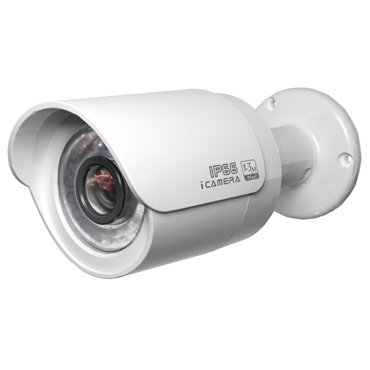
\includegraphics[width=0.9\linewidth]{dahua-hw2100}
\end{subfigure}
\begin{subfigure}{0.4\textwidth}
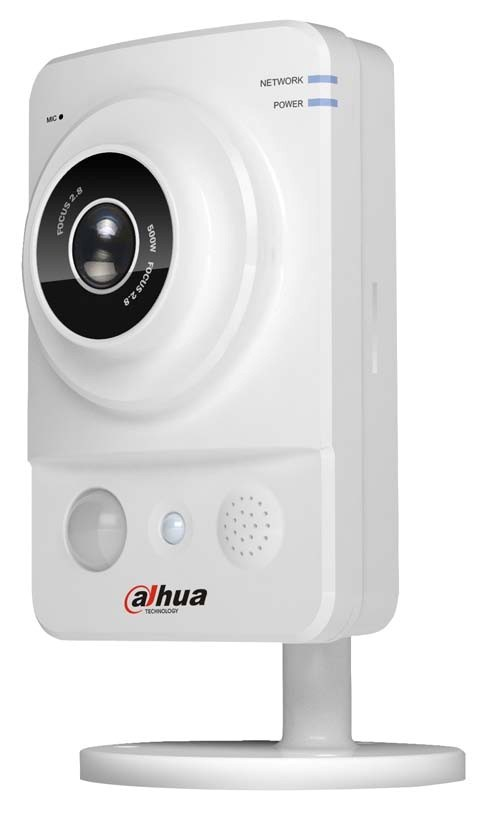
\includegraphics[width=0.5\linewidth]{dahua-k100}
\end{subfigure}


\caption{Cámaras Dahua: HFW2100 (izquierda) y K100 (derecha) \protect\cite{dahua2016-iu}}
\label{fig:dahua-cam}
\end{figure}

    % \begin{figure}
    %     \centering
    %     % \includegraphics[width=0.85\textwidth]
    %     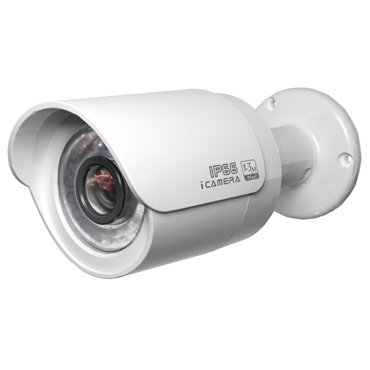
\includegraphics[scale=0.3,valign=t]{dahua-hw2100}

    % \end{figure}
Algunas de sus caracteristicas de la IPC-K100 incluyen:
\begin{itemize}
\item 1/3” 1.3 Megapixel Aptina CMOS
\item H.264 \& MJPEG codificación de doble-flujo
\item Max 15fps@1.3M(1280×960)/25/30fps@720P(1280×720)
\item DWDR, Dia/Noche, 2DNR, Auto iris, AWB, AGC, BLC
\item Monitoreo en múltiples redes: Visor web, CMS(DSS/PSS) \& DMSS
\item Lente 3.6mm fijo
\item LEDs Blancos de 10m de longitud 
\item Sensor PIR con rango de 6m
\item Memoria Micro SD, PoE, Wi-Fi 
\item Protocolos: IPv4/IPv6, HTTP, SSL, TCP/IP, UDP, UPnP, ICMP, IGMP, SNMP, RTSP, RTP, SMTP, NTP, DHCP, DNS, PPPOE, DDNS, FTP,  IP Filter,  QoS, Bonjou
\end{itemize}



\chapter{Estructura de un Proyecto Laravel}
La capa de presentación consiste en vistas y controladores que solicitan información a los servicios externos, a los cuales acceden a través de sus APIs.
\clearpage
La estructura de un proyecto de Laravel consiste en:

\vspace{0.5cm}
{\setstretch{1.0}
\dirtree{%
.1 project/.
    .2 \vdots.
    .2 app/.
        .3 \vdots.
        .3 Http/.
            .4 Controllers/.
                .5 CamaraController.php.
                .5 Controller.php.
                .5 LugarController.php.
                .5 \vdots.
            .4 Requests/.
            .4 Kernel.php.
            .4 routes.php.
    .2 config/.
        .3 \vdots.
        .3 app.php.
        .3 database.php.
        .3 compile.php.
    .2 database/.
        .3 \vdots.
        .3 migrations.
    .2 public/. 
        .3 css.
        .3 fonts.
        .3 js.
        .3 \vdots.
    .2 resources/.
        .3 \vdots.
        .3 views.
    .2 vendor/.
    .2 .env.
    .2 \vdots.
    .2 composer.json.
}
}
Donde:

\begin{itemize}
\item \textit{app/} contiene los controladores correspondientes a cada servicio.
\item \textit{config/} contiene la configuración de la aplicación, base de datos, vistas, compilación, etc..
\item \textit{database/} contiene los archivos necesarios para realizar las migraciones de la base de datos, simplificadas con la herramienta Artisan de Laravel \footnote{\url{https://laravel.com/docs/5.3/artisan}}.
\item \textit{public/} contiene las configuraciones de CSS, fuentes y Javascript, además del archivo de la pagina principal index.php.
\item \textit{resources/} contiene las vistas que se presentan al usuario.
\item \textit{vendor/} contiene todos los componentes que incluye Laravel.
\item \textit{.env y composer.json} describen las variables de entorno y las dependencias necesarias para ejecutar la aplicación respectivamente.

\end{itemize}

\newpage
\chapter{Diagrama de Paquetes}
\label{appendix:paquetes}
A continuación se adjunta un diagrama de paquetes del PFG, como alternativa para representar la distribución de las clases en el modelo conceptual.
\begin{landscape}

        \begin{figure}[H]
        \centering
        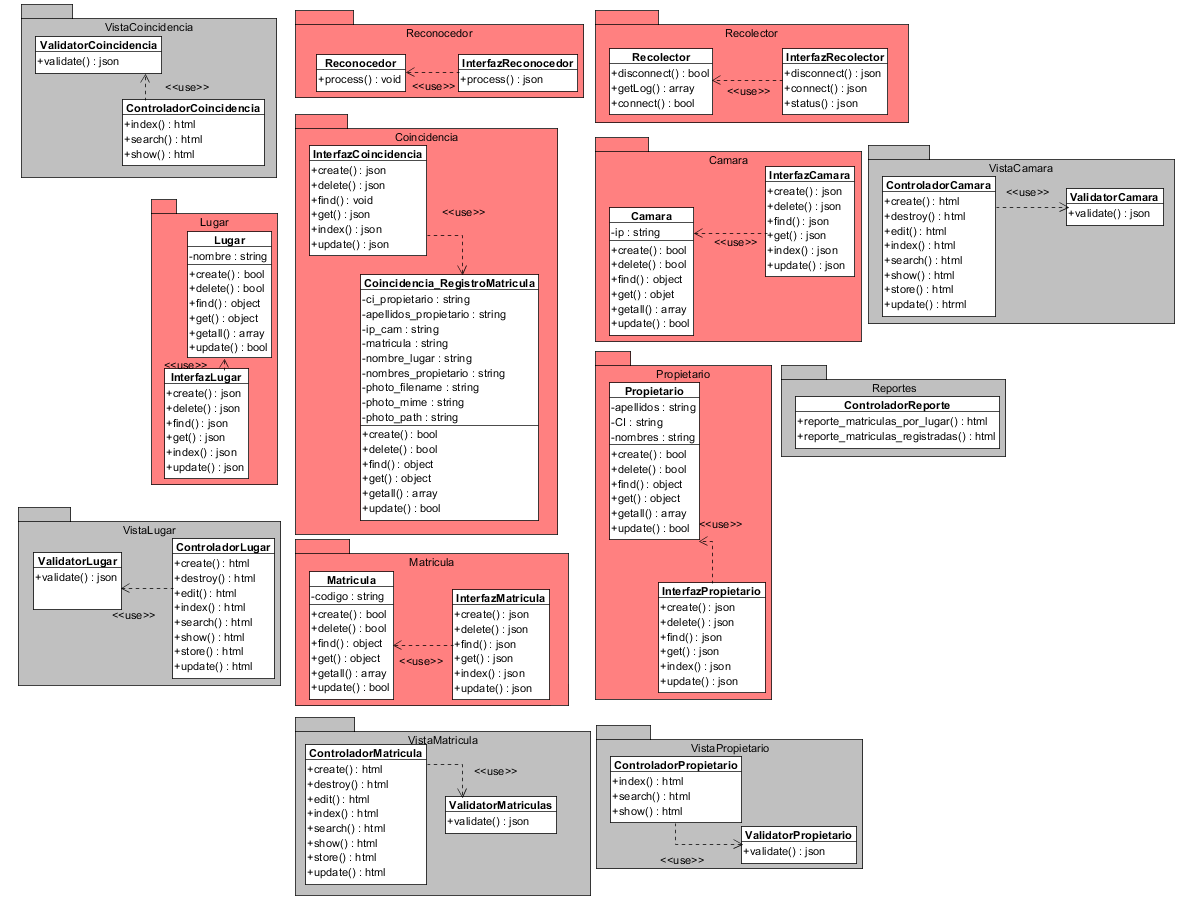
\includegraphics[width=1.1\textwidth]{class-packages-extended}
        \caption{Modelo Conceptual - Detalle}
        \label{fig:CLASS-brief}
    \end{figure}
\end{landscape}

     \begin{figure}[H]
        \centering
        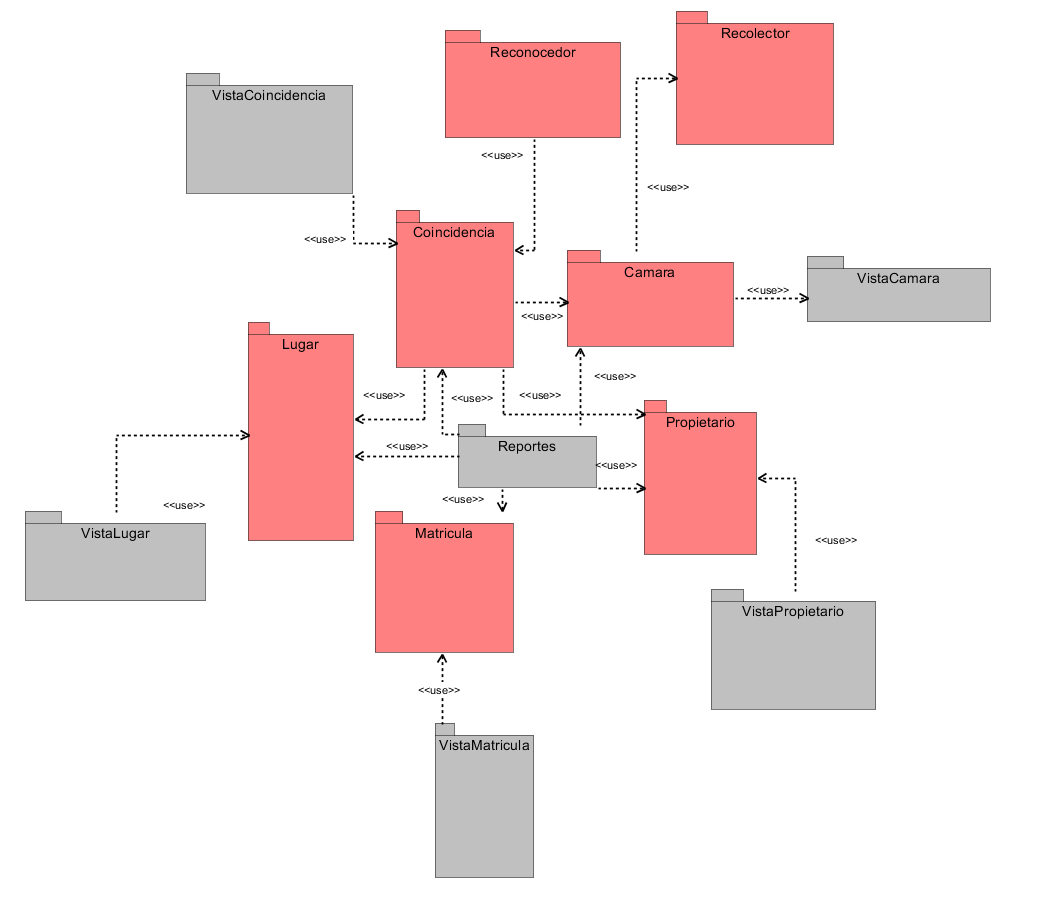
\includegraphics[width=1\textwidth]{class-packages}
        \caption{Modelo Conceptual - Paquetes}
        \label{fig:CLASS-crop}
    \end{figure}
    

\chapter{ALPR en Ambientes Abiertos}
A pesar de que la detección de matrículas se considera un problema resuelto, los algoritmos existentes funcionan óptimamente bajo condiciones controladas. Por ejemplo, algunos sistemas requieren hardware sofisticado para la grabación de video, luces infrarrojas, o algunos son estrictos con respecto al ángulo en que se observa la matrícula. En este sentido, sigue siendo un desafío la detección de matrículas en ambientes abiertos.

Los módulos ALPR deben operar con la suficiente rapidez como para no perder ningún objeto de interés en una escena. Sin embargo, con el crecimiento exponencial del poder de procesamiento los últimos avances operan en menos de 50ms para la detección y el reconocimiento de matriculas (procesando mas de 20 cuadros por segundo en videos) \cite{Anagnostopoulos2008-uh}.

Generalmente, se debe resolver dos problemas: detectar dónde se encuentra la matrícula y su tamaño. En esto participan los diversos factores que obstaculizan la detección, como los ángulos de observación del a cámara, los objetos del fondo, matrículas de diferente tamaño, imagen de calidad pobre, condiciones de luz variantes y detección de múltiples matrículas \cite{zhou2012}

\pagebreak
\chapter{Interpolación Bilineal}
El algoritmo LBP utiliza la interpolación bilineal para obtener el valor/código LBP en puntos que están fuera de un píxel. 

En la interpolación bilineal, si se quiere encontrar el valor para la función f desconocida en el punto \(P = (x, y)\) y conociendo el valor de f en los cuatro puntos \(Q11 = (x1, y1), Q12 = (x1, y2)\), \(Q21 = (x2, y1)\) y \(Q22 = (x2, y2)\).

Se puede encontrar el valor LBP interpolando linealmente en una dirección y después en la otra. Existen otras maneras de resolver la interpolación bilineal \cite{Banerjee2014-xj}.

\pagebreak
\chapter{Etcd}
Etcd \cite{CoreOS2016-cp} es un registro distribuido y consistente de llaves  y valores, para el almacenamiento de configuración compartida y descubrimiento de servicios en un cluster de maquinas (y es utilizado por Kubernetes).
    \begin{figure}[H]
        \centering
        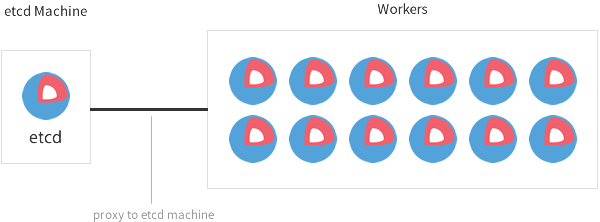
\includegraphics[width=0.9\textwidth]{etcd}
        \caption{Cluster CoreOS con Etcd \protect\cite{CoreOS2016-zr}}
        \label{fig:coreos2016-etcd}
    \end{figure}
    \pagebreak
Características:
\begin{itemize}
\item Soporta una API para el usuario, TLS\footnote{Transport Layer Security es un protocolo criptográfico para las comunicaciones a través de una red.} automático y autenticación con certificados.
\item Comunicación utilizando un algoritmo de consenso de Raft\footnote{\url{https://raft.github.io/}}.
\item Escritura y lectura con curl.
\item Almacenar datos en directorios
\item Observar cambios en una llave y reaccionar ante ellos.


\end{itemize}
\pagebreak
\chapter{Cloudify: Proyecto ARIA}
El proyecto ARIA es una plataforma y un conjunto de herramientas para validar y crear instancias de servicios basados en plantillas TOSCA. Utiliza una API para Python, una API RESTful y puede ser desplegado como  microservicio \cite{Cloudify2016-cl}.
Incluye las siguientes validaciones:
\begin{itemize}
\item \textbf{Errores de plataforma:} red, hardware, etc.
\item \textbf{Errores de sintaxis y formato:} YAML, XML, JSON.
\item \textbf{Validación de datos:} Asignación de una cadena donde se espera un entero, etc.
\item \textbf{Relación entre tipos:} referencias a tipos desconocidos, bucles de herencia de tipos.
\item \textbf{Dependencias externas:} fallas debido a ausencia de recursos externos; por ejemplo, la falta de una máquina virtual valida, credenciales para una API, etc.

\end{itemize}
